\section[Identification et représentation des besoins]{Identification et représentation des besoins}    
    \subsection[Identification des acteurs]{Identification des acteurs}
    Voici les acteurs identifiés dans le cadre de notre
    travail :
    \par
        \begin{itemize}
            \setlength{\itemsep}{0pt}
            \item [\ding{226}] \textbf{L’internaute} : est celui qui visite
            notre plateforme sans y être inscrit.
            \item [\ding{226}] \textbf{Le client} : est celui qui a créé un compte
            utilisateur dans le système.
            \item [\ding{226}] \textbf{Le guichetier} : est celui qui vend le ticket de bus.
            \item [\ding{226}] \textbf{Le contrôleur} : est celui qui vérifie la validité
            du ticket de bus avant que le client ne puisse effectuer son voyage.
            \item [\ding{226}] \textbf{L’administrateur} : il est chargé de
            monitorer le système afin d’éviter tout débordement des utilisateurs,
            et voir tous les mauvais fonctionnements du système et les régler
            à distance.
            \item [\ding{226}] \textbf{Le manager} : est celui qui utilise le système
            pour visualiser le tableau de bord et consulter le rapport. 
        \end{itemize}
    \subsection[Identification des cas d’utilisation]{Identification des cas d’utilisation}
    Les cas d’utilisations ou fonctionnalités de notre
    système sont les suivants :
    \par
        \begin{enumerate}
            \setlength{\itemsep}{0pt}
            \item Créer compte
            \item S’authentifier
            \item Consulter avis
            \item Consulter notification
            \item Scanner ticket
            \item Donner avis
            \item Envoyer message
            \item Vendre ticket
            \item Gérer comptes
            \item Gérer voyages
            \item Génère tableau de bord
            \item Consulter tableau de bord
            \item Consulter rapport
        \end{enumerate}
    Chacun des cas figurant dans la liste présenter
    ci-haut, seras expliquer plus en détaille dans
    sa description textuelle.
\pagebreak
    \subsection[Diagrammes de cas d’utilisation]{Diagrammes de cas d’utilisation}
    Après avoir eu à identifier les acteurs et leurs cas d’utilisation
    voici comment se présente le diagramme de cas d’utilisation :
        \begin{figure}[H]
            \centering
            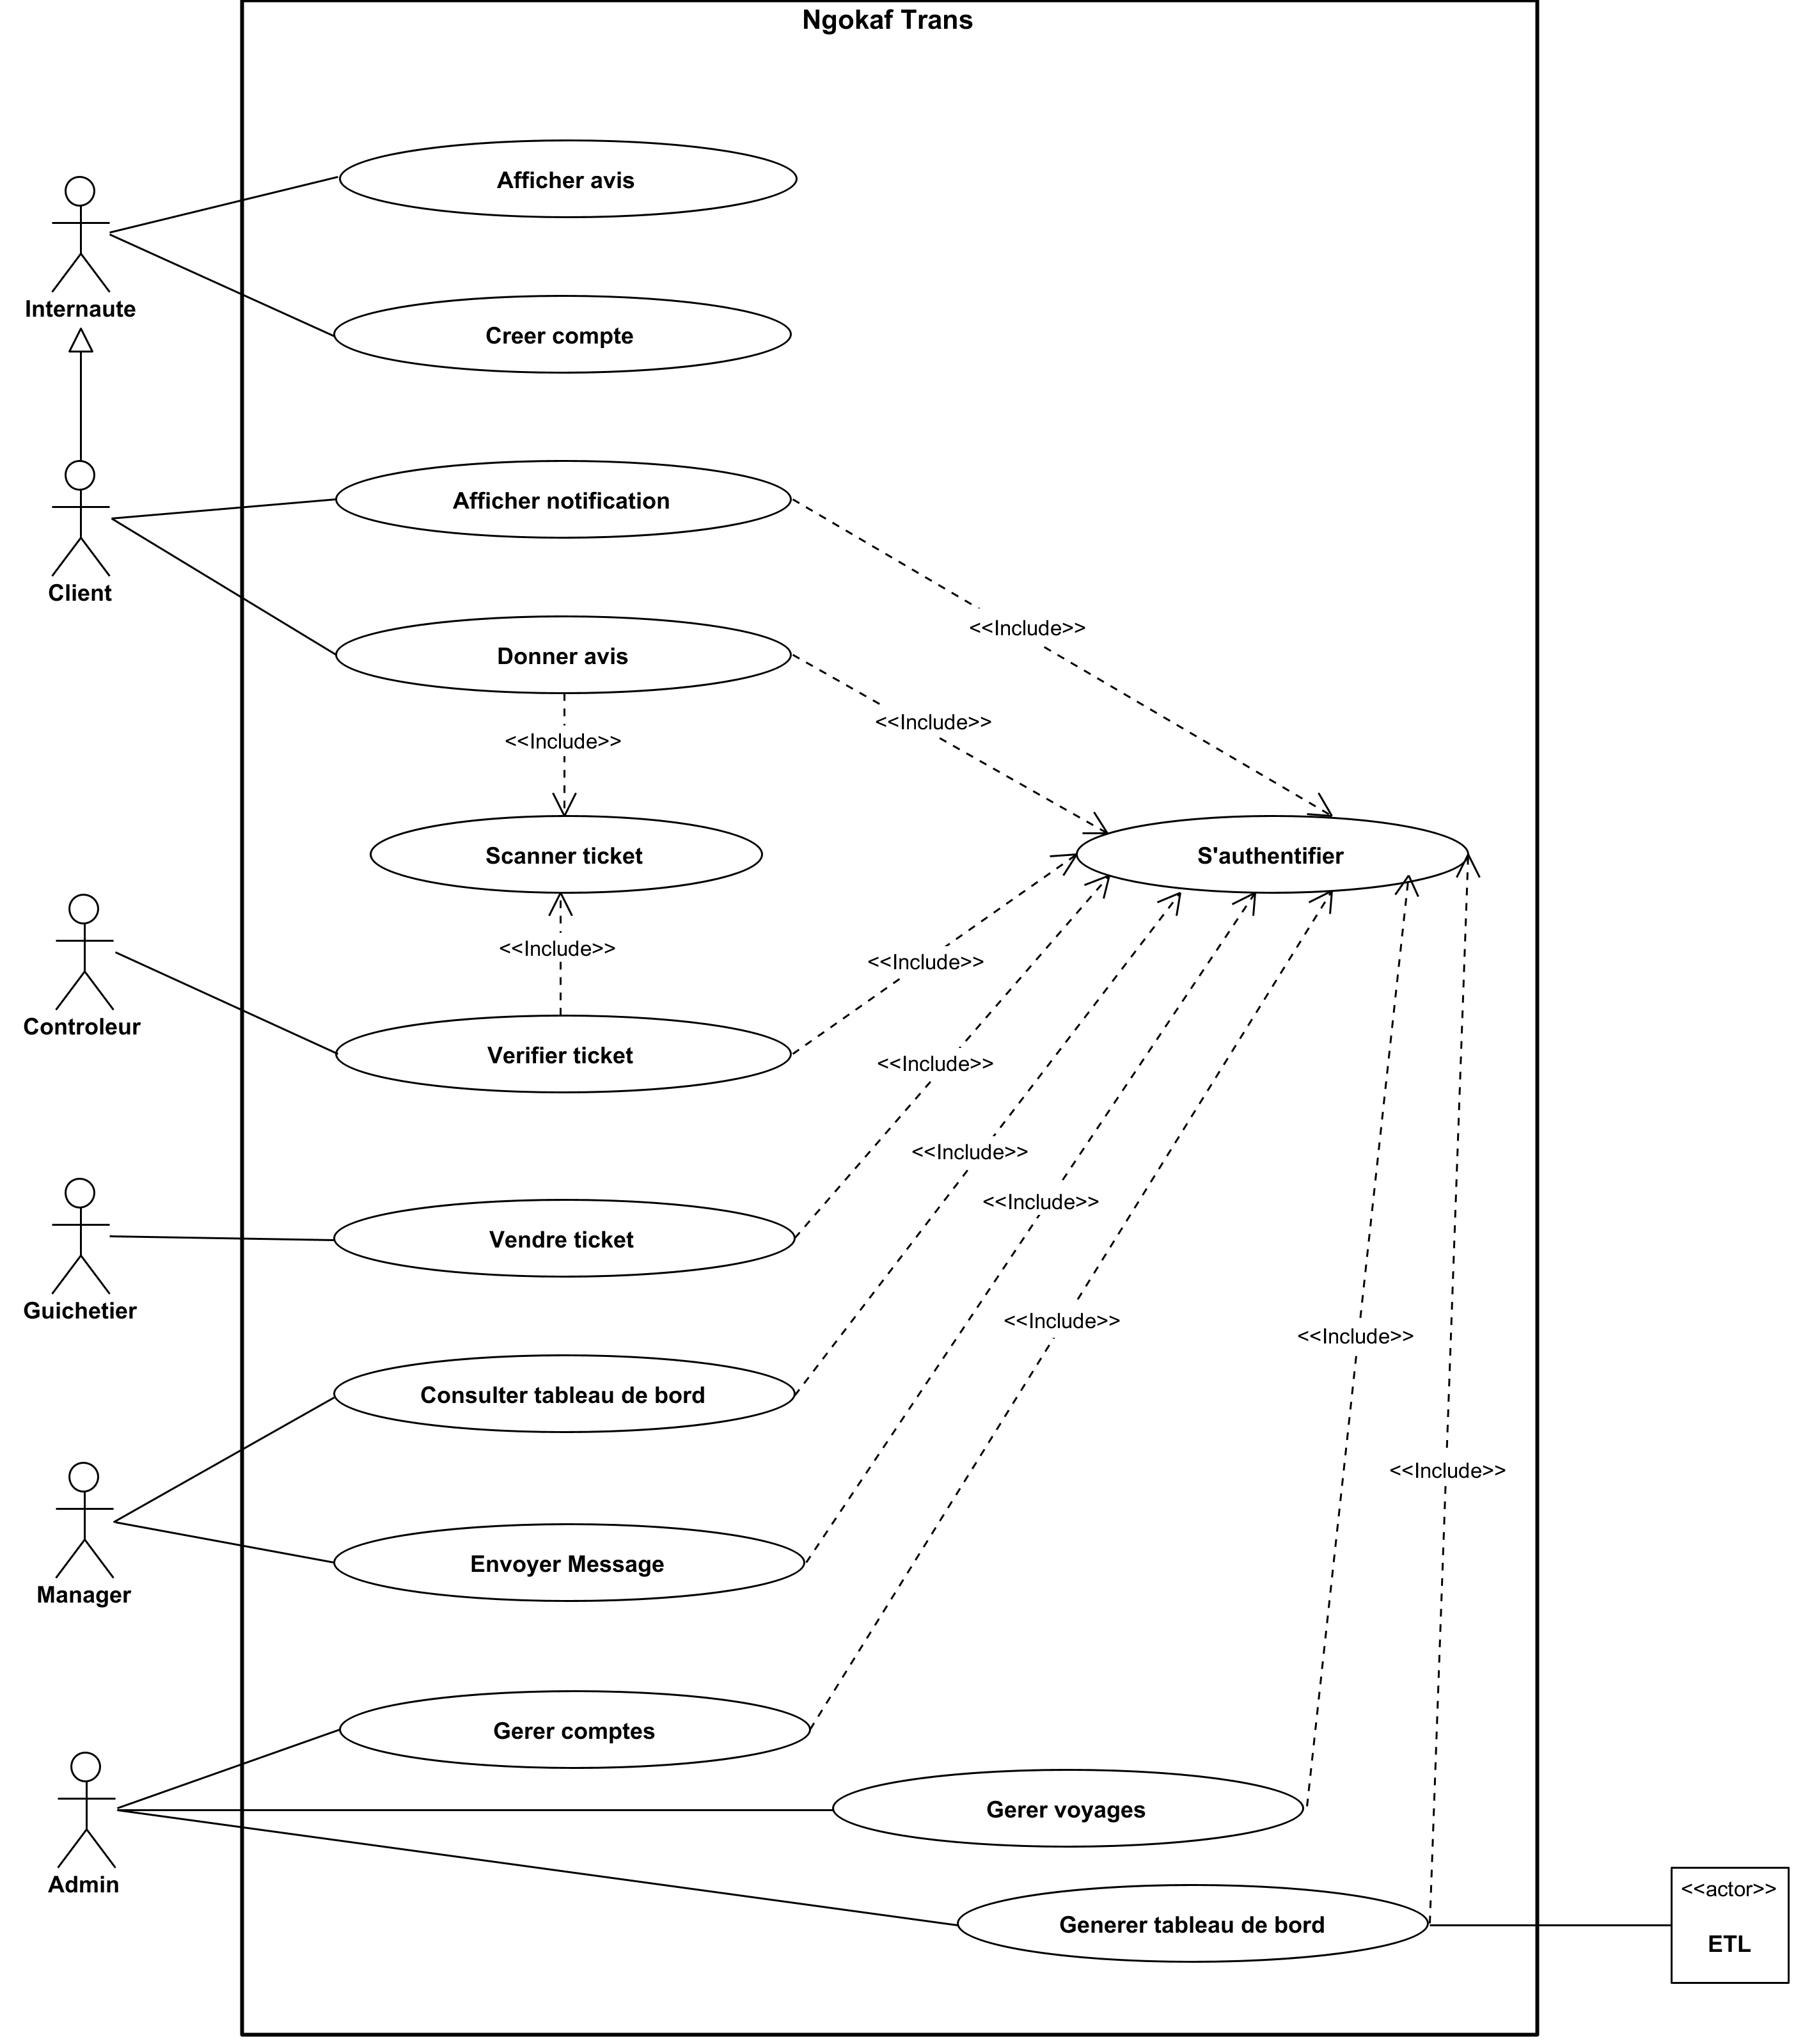
\includegraphics[width=150mm]{images/diagramme-de-cu/use-case.png}
            \caption{Diagramme de cas d’utilisation}
            \label{fig:dcu}
        \end{figure}
\pagebreak